\clearpage
\phantomsection
\label{202501121340}
\renewcommand{\notetitle}{Question 2}

\section*{Note Information}
\begin{itemize}
  \item \textbf{ID:} \texttt{202501121340}
  \item \textbf{Timestamp:} \texttt{\today \ \currenttime}
  \item \textbf{Tags:} \texttt{Tutoring, Chhean, Session-1}
  \item \textbf{References:}
    \begin{itemize}
      \item \href{}{}
    \end{itemize}
\end{itemize}


\section*{Main Content}
\textbf{Main Idea}\\
Suppose a particle is moving on the $x$-axis between the time $t=0$ seconds and $t = 9$ seconds. Its initial position at $t=0$ seconds is $x(0)=2$ meters. 
The velocity-time graph of the motion is shown below.\\
\begin{center}
  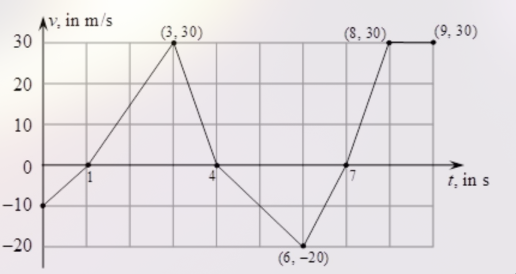
\includegraphics[width=0.5\textwidth]{Figures/Question-2.png}\\
\end{center}
On the $x$-axis, the abscissa of the farthest point to the right of the origin that the particle reaches over the time interval $0 \leq t \leq 9$ seconds is 42 meters.\\

\textbf{Explanation}\\
By looking at the graph, we notice that the velocity is positive on the intervals $1 \leq t \leq 4$ and $7 \leq t \leq 9$. The velocity is negative on the intervals $0 \leq t \leq 1$ and $4 \leq t \leq 7$.
The area under the curve between $t = 1$ and $t=4$ is calculated by finding the area of the triangle with base 3 and height 30:
\begin{align*}
  A_1 &= \frac{1}{2} \cdot 3 \cdot 30 = 45
\end{align*}
The area under the curve for the other three intervals are computed in a similar way below:
\begin{align*}
  A_2 &= \frac{1}{2} \cdot 1 \cdot 30 + 1 \cdot 30 = 30\\
  A_3 &= \frac{1}{2} \cdot 1 \cdot 10 = 5\\
  A_4 &= \frac{1}{2} \cdot 3 \cdot 20 = 30\\
\end{align*}
Using the areas above, we can compute $x(t)$ at key times, using the fact that $x(t) = x(0) + \int_0^t v(t) dt$:\\
At $t=1$:
\begin{align*}
  x(1) &= x(0) - A_3 = 2 - 5 = -3\\
\end{align*}
At $t = 4$:
\begin{align*}
  x(4) &= x(1) + A_1 = -3 + 45 = 42\\
\end{align*}
At $t = 7$:
\begin{align*}
  x(7) &= x(4) - A_4 = 42 - 30 = 12\\
\end{align*}
At $t = 9$:
\begin{align*}
  x(9) &= x(7) - A_2 = 12 + 30 = 42\\
\end{align*}
The particle is farthest to the right at $t = 4$ and $t = 9$, where:
\begin{align*}
  x_{max} = 42 \text{ meters}
\end{align*}

\section*{Review}
\begin{enumerate}
  \item 
\end{enumerate}


\section*{Links to Other Notes}
\begin{itemize}
  \item \hyperref[]{}
\end{itemize}

\section*{Table of Contents}

\begin{itemize}
  \item \hyperref[toc]{TOC}
\end{itemize}

